% Options for packages loaded elsewhere
\PassOptionsToPackage{unicode}{hyperref}
\PassOptionsToPackage{hyphens}{url}
%
\documentclass[
]{book}
\usepackage{amsmath,amssymb}
\usepackage{lmodern}
\usepackage{ifxetex,ifluatex}
\ifnum 0\ifxetex 1\fi\ifluatex 1\fi=0 % if pdftex
  \usepackage[T1]{fontenc}
  \usepackage[utf8]{inputenc}
  \usepackage{textcomp} % provide euro and other symbols
\else % if luatex or xetex
  \usepackage{unicode-math}
  \defaultfontfeatures{Scale=MatchLowercase}
  \defaultfontfeatures[\rmfamily]{Ligatures=TeX,Scale=1}
\fi
% Use upquote if available, for straight quotes in verbatim environments
\IfFileExists{upquote.sty}{\usepackage{upquote}}{}
\IfFileExists{microtype.sty}{% use microtype if available
  \usepackage[]{microtype}
  \UseMicrotypeSet[protrusion]{basicmath} % disable protrusion for tt fonts
}{}
\makeatletter
\@ifundefined{KOMAClassName}{% if non-KOMA class
  \IfFileExists{parskip.sty}{%
    \usepackage{parskip}
  }{% else
    \setlength{\parindent}{0pt}
    \setlength{\parskip}{6pt plus 2pt minus 1pt}}
}{% if KOMA class
  \KOMAoptions{parskip=half}}
\makeatother
\usepackage{xcolor}
\IfFileExists{xurl.sty}{\usepackage{xurl}}{} % add URL line breaks if available
\IfFileExists{bookmark.sty}{\usepackage{bookmark}}{\usepackage{hyperref}}
\hypersetup{
  pdftitle={Advanced decision modelling in the context of Health Technology Assessment},
  pdfauthor={Juan Pablo Diaz Martinez},
  hidelinks,
  pdfcreator={LaTeX via pandoc}}
\urlstyle{same} % disable monospaced font for URLs
\usepackage{color}
\usepackage{fancyvrb}
\newcommand{\VerbBar}{|}
\newcommand{\VERB}{\Verb[commandchars=\\\{\}]}
\DefineVerbatimEnvironment{Highlighting}{Verbatim}{commandchars=\\\{\}}
% Add ',fontsize=\small' for more characters per line
\usepackage{framed}
\definecolor{shadecolor}{RGB}{248,248,248}
\newenvironment{Shaded}{\begin{snugshade}}{\end{snugshade}}
\newcommand{\AlertTok}[1]{\textcolor[rgb]{0.94,0.16,0.16}{#1}}
\newcommand{\AnnotationTok}[1]{\textcolor[rgb]{0.56,0.35,0.01}{\textbf{\textit{#1}}}}
\newcommand{\AttributeTok}[1]{\textcolor[rgb]{0.77,0.63,0.00}{#1}}
\newcommand{\BaseNTok}[1]{\textcolor[rgb]{0.00,0.00,0.81}{#1}}
\newcommand{\BuiltInTok}[1]{#1}
\newcommand{\CharTok}[1]{\textcolor[rgb]{0.31,0.60,0.02}{#1}}
\newcommand{\CommentTok}[1]{\textcolor[rgb]{0.56,0.35,0.01}{\textit{#1}}}
\newcommand{\CommentVarTok}[1]{\textcolor[rgb]{0.56,0.35,0.01}{\textbf{\textit{#1}}}}
\newcommand{\ConstantTok}[1]{\textcolor[rgb]{0.00,0.00,0.00}{#1}}
\newcommand{\ControlFlowTok}[1]{\textcolor[rgb]{0.13,0.29,0.53}{\textbf{#1}}}
\newcommand{\DataTypeTok}[1]{\textcolor[rgb]{0.13,0.29,0.53}{#1}}
\newcommand{\DecValTok}[1]{\textcolor[rgb]{0.00,0.00,0.81}{#1}}
\newcommand{\DocumentationTok}[1]{\textcolor[rgb]{0.56,0.35,0.01}{\textbf{\textit{#1}}}}
\newcommand{\ErrorTok}[1]{\textcolor[rgb]{0.64,0.00,0.00}{\textbf{#1}}}
\newcommand{\ExtensionTok}[1]{#1}
\newcommand{\FloatTok}[1]{\textcolor[rgb]{0.00,0.00,0.81}{#1}}
\newcommand{\FunctionTok}[1]{\textcolor[rgb]{0.00,0.00,0.00}{#1}}
\newcommand{\ImportTok}[1]{#1}
\newcommand{\InformationTok}[1]{\textcolor[rgb]{0.56,0.35,0.01}{\textbf{\textit{#1}}}}
\newcommand{\KeywordTok}[1]{\textcolor[rgb]{0.13,0.29,0.53}{\textbf{#1}}}
\newcommand{\NormalTok}[1]{#1}
\newcommand{\OperatorTok}[1]{\textcolor[rgb]{0.81,0.36,0.00}{\textbf{#1}}}
\newcommand{\OtherTok}[1]{\textcolor[rgb]{0.56,0.35,0.01}{#1}}
\newcommand{\PreprocessorTok}[1]{\textcolor[rgb]{0.56,0.35,0.01}{\textit{#1}}}
\newcommand{\RegionMarkerTok}[1]{#1}
\newcommand{\SpecialCharTok}[1]{\textcolor[rgb]{0.00,0.00,0.00}{#1}}
\newcommand{\SpecialStringTok}[1]{\textcolor[rgb]{0.31,0.60,0.02}{#1}}
\newcommand{\StringTok}[1]{\textcolor[rgb]{0.31,0.60,0.02}{#1}}
\newcommand{\VariableTok}[1]{\textcolor[rgb]{0.00,0.00,0.00}{#1}}
\newcommand{\VerbatimStringTok}[1]{\textcolor[rgb]{0.31,0.60,0.02}{#1}}
\newcommand{\WarningTok}[1]{\textcolor[rgb]{0.56,0.35,0.01}{\textbf{\textit{#1}}}}
\usepackage{longtable,booktabs,array}
\usepackage{calc} % for calculating minipage widths
% Correct order of tables after \paragraph or \subparagraph
\usepackage{etoolbox}
\makeatletter
\patchcmd\longtable{\par}{\if@noskipsec\mbox{}\fi\par}{}{}
\makeatother
% Allow footnotes in longtable head/foot
\IfFileExists{footnotehyper.sty}{\usepackage{footnotehyper}}{\usepackage{footnote}}
\makesavenoteenv{longtable}
\usepackage{graphicx}
\makeatletter
\def\maxwidth{\ifdim\Gin@nat@width>\linewidth\linewidth\else\Gin@nat@width\fi}
\def\maxheight{\ifdim\Gin@nat@height>\textheight\textheight\else\Gin@nat@height\fi}
\makeatother
% Scale images if necessary, so that they will not overflow the page
% margins by default, and it is still possible to overwrite the defaults
% using explicit options in \includegraphics[width, height, ...]{}
\setkeys{Gin}{width=\maxwidth,height=\maxheight,keepaspectratio}
% Set default figure placement to htbp
\makeatletter
\def\fps@figure{htbp}
\makeatother
\setlength{\emergencystretch}{3em} % prevent overfull lines
\providecommand{\tightlist}{%
  \setlength{\itemsep}{0pt}\setlength{\parskip}{0pt}}
\setcounter{secnumdepth}{5}
\usepackage{booktabs}
\ifluatex
  \usepackage{selnolig}  % disable illegal ligatures
\fi
\usepackage[]{natbib}
\bibliographystyle{apalike}

\title{Advanced decision modelling in the context of Health Technology Assessment}
\author{Juan Pablo Diaz Martinez}
\date{2021-11-19}

\begin{document}
\maketitle

{
\setcounter{tocdepth}{1}
\tableofcontents
}
\hypertarget{introduction}{%
\chapter*{Introduction}\label{introduction}}
\addcontentsline{toc}{chapter}{Introduction}

Bringing a new health technology to market and into the hands of a patient is a long process. Most of the times patients, who have a medical need, ask themselves why does it take so long to make the health technology available to everyone. When a health technology is in the market, it usually took between 5 to 10 years to make
it available.

Depending on the country, governments usually are involved in the reimbursement process. They usually ask the next questions when a new health technology is available:

\begin{itemize}
\tightlist
\item
  How much does it cost?
\item
  Will it save lives and/or improve quality of life?
\item
  Do we have enough budget to fund it?
\item
  If we have a pool of interventions for a specific disease, which one/ones should we reimburse?
\end{itemize}

Moreover, physicians, patients, insurance plans, and advocacy groups play an important role when new technologies are available in the market (why?). Even though a new technology see the light (i.e.~it has proved to be safe and effective), insurance providers or the government will not necessarily cover it. Usually they argue that the new technology is ``Not cost-effective'' or ``Not have good value for money''. \emph{These notes aim to provide all the necessary tools to decide if a new intervention has a good value-for-money.} It is important to stress that value-for-money decision is only one of many questions that are asked by one of the users of a \textbf{health technology assessment (HTA)}: patients, healthcare workers, government, and others.

\hypertarget{why-reimbursment-submissions-fail}{%
\section*{Why reimbursment submissions fail?}\label{why-reimbursment-submissions-fail}}
\addcontentsline{toc}{section}{Why reimbursment submissions fail?}

According to \citet{goeree2015health}, the reasons for rejection are:

\begin{enumerate}
\def\labelenumi{\arabic{enumi}.}
\tightlist
\item
  Inappropriate comparator. Lack of proper statistical analysis.
\item
  Inappropriate outcome. Use of surrogates.
\item
  Inappropriate analysis. Lack of robust evidence for costs and quality of life.
\item
  High cost to the government.
\end{enumerate}

\hypertarget{topics-of-the-course}{%
\section*{Topics of the course}\label{topics-of-the-course}}
\addcontentsline{toc}{section}{Topics of the course}

\begin{enumerate}
\def\labelenumi{\arabic{enumi}.}
\tightlist
\item
  What is HTA?
\item
  Introduction to decision-analytic models
\item
  Good practices in decision modelling
\item
  Evidence-based medicine
\item
  Decision tree-models
\item
  State-transition models with the Markov assumption
\item
  Partitioned survival models
\item
  Microsimulation
\item
  Discrete-event simulation
\item
  Uncertainty and decision-making
\item
  Presentation of results
\end{enumerate}

\hypertarget{statistical-computing}{%
\section*{Statistical computing}\label{statistical-computing}}
\addcontentsline{toc}{section}{Statistical computing}

The use of open-source programming languages, such as \texttt{R}, in health decision sciences is growing and has the potential to facilitate model transparency, reproducibility, and shareability. However, realizing this potential can be challenging. Models are complex and primarily built to answer a research question, with model sharing and transparency relegated to being secondary goals. Moreover, many decision modelers are not formally trained in computer programming and may lack good coding practices, further compounding the problem of model transparency. \textbf{Therefore, throughout this course, the programming language \texttt{R} will be used to show its potential for advanced modelling in the context of HTA.}

For this course, we will be using the book \href{https://r4ds.had.co.nz/}{``R for Data Science''}. To install \texttt{R} and \texttt{Rstudio}, instructions are provided in Chapter 1 of this book. We will also use Excel throughout this course.

\hypertarget{evaluation}{%
\section*{Evaluation}\label{evaluation}}
\addcontentsline{toc}{section}{Evaluation}

\begin{longtable}[]{@{}ccc@{}}
\toprule
Item & Percentage & Due date \\
\midrule
\endhead
Assignment 1 & 15\% & Nov 27, 2021 \\
Assignment 2 & 15\% & Dec 23, 2021 \\
Take-home exam & 30\% & Jan 7, 2022 \\
Project proposal & 5\% & Nov 22, 2021 \\
Project presentation & 5\% & Jan 14, 2022 \\
Final project & 30\% & Jan 17, 2022 \\
\bottomrule
\end{longtable}

The intent is to allow the students to demonstrate their mastery of this class through the following way. \textbf{Project proposal, presentation and final project will be done in pairs}.

\hypertarget{asssignments}{%
\subsection*{Asssignments}\label{asssignments}}
\addcontentsline{toc}{subsection}{Asssignments}

The assignments are handed out approximately two weeks prior to the due date. Late work will not be marked, with the exception of an advance permission from the instructor.

\hypertarget{project-proposal}{%
\subsection*{Project proposal}\label{project-proposal}}
\addcontentsline{toc}{subsection}{Project proposal}

(1 page)

The final deliverable for this course is a mini-HTA on a medical technology (preferably something topical), with a focus on the quantitative aspect of it. Given that the translation of a health policy question into a relevant research question is an essential first step in the conduct of HTA, students are required to formulate a research question and submit for grading purposes. This should include at leas some of the following: an overview of the technology being assessed; a clear specification of the policy problem; and the research question(s) (including PICO) with objectives.

\hypertarget{project-presentation}{%
\subsection*{Project presentation}\label{project-presentation}}
\addcontentsline{toc}{subsection}{Project presentation}

(20 minutes with extra 5 minutes for questions)

Students will be expected to present their final course paper and answer questions. Student will be graded on their presentations.

\hypertarget{final-project}{%
\subsection*{Final project}\label{final-project}}
\addcontentsline{toc}{subsection}{Final project}

(20 pages double-spaced)

The main assignment will require students to produce a scaled down HTA, with a focus on the quantitative aspect of it. The objective of the final project is for the student to show that they have obtained a clear understanding of the advanced methods in decision modelling in the context of HTA. More information will be provided throughout the course, but the paper should contain the following:

\begin{enumerate}
\def\labelenumi{\alph{enumi})}
\tightlist
\item
  Background and technology overview
\item
  Formulation of the question you are trying to answer through your mini-HTA
\item
  Review of the clinical literature
\item
  Description of the structure of the model
\item
  Description of the function of the model
\item
  Results
\item
  Conclusions
\end{enumerate}

\hypertarget{bibliography}{%
\section*{Bibliography}\label{bibliography}}
\addcontentsline{toc}{section}{Bibliography}

\emph{Briggs, A., Sculpher, M., \& Claxton, K. (2006). Decision modelling for health economic evaluation. Oxford University Press.}

\emph{Gray, A. M., Clarke, P. M., Wolstenholme, J. L., \& Wordsworth, S. (2011). Applied methods of cost-effectiveness analysis in healthcare (Vol. 3). Oxford University Press.}

\emph{Edlin, R., McCabe, C., Hulme, C., Hall, P., \& Wright, J. (2015). Cost effectiveness modelling for health technology assessment: a practical course. Springer.}

\hypertarget{HTA}{%
\chapter{What is HTA?}\label{HTA}}

\hypertarget{pre-session-readings}{%
\section{Pre-session readings}\label{pre-session-readings}}

\emph{Goodman, C. S. (2004). Introduction to health technology assessment. The Lewin Group. virginia, USA.} \href{https://www.nlm.nih.gov/nichsr/hta101/ta10101.html}{link}. Chapters 1, 2, and 5.

\emph{Briggs, A., Sculpher, M., \& Claxton, K. (2006). Decision modelling for health economic evaluation. Oxford University Press.} Chapter 1.

Chapters 1 and 2 of \emph{R for data science}.

\hypertarget{definition-and-rationale}{%
\section{Definition and rationale}\label{definition-and-rationale}}

The first thing that we need to know is the definition of a \textbf{health technology}. A health technology is any intervention that may be used to promote health, to prevent, diagnose or treat disease or for rehabilitation or long-term care.

\textbf{Questions}

\begin{enumerate}
\def\labelenumi{\arabic{enumi}.}
\tightlist
\item
  List some examples of health technologies.
\end{enumerate}

Depending on the agency, health technology assessment has a broad spectrum of definitions:

\emph{``HTA is a multidisciplinary process that uses explicit methods to determine the value of a health technology at different points in its lifecycle. The purpose is to inform decision-making in order to promote an equitable, efficient, and high-quality health system.'' \href{https://www.inahta.org/}{INAHTA}}

\emph{``Health technology assessment is a multidisciplinary process that uses explicit methods to determine the value of a health technology at different points in its lifecycle. The purpose is to inform decision-making in order to promote an equitable, efficient, and high-quality health system.'' \href{https://www.eunethta.eu/}{EUnetHTA}}

\emph{``A comprehensive, objective, evidence-based analysis of the clinical effectiveness, cost-effectiveness and broader impact of drugs, medical technologies and health systems. HTA examines technologies at all stages of their life cycle, from development through to maturity and obsolescence.'' \href{https://www.cadth.ca}{CADTH}}

The purpose of HTA is to support/help decision makers by identifying technologies that will improve health outcomes and deliver value for every dollar invested.

\begin{itemize}
\tightlist
\item
  Does a new health technology offer a clinical advantage over the alternatives/standard approaches?
\item
  Is it worth the investment?
\item
  Can I pay for it?
\item
  Who would benefit from it?
\item
  Any ethical, social or legal issues
\end{itemize}

But, what are the reasons for conducting HTAs?

\begin{itemize}
\tightlist
\item
  Increased demand for healthcare (why?)
\item
  Soaring healthcare costs
\item
  Increased rate of diffusion of new technologies and associated evidence
\end{itemize}

\begin{figure}

{\centering 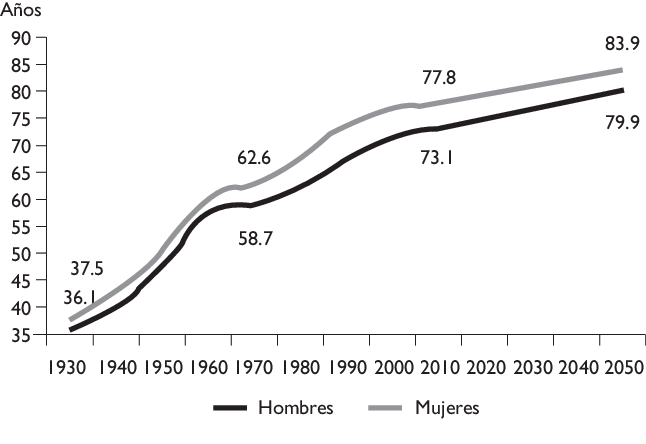
\includegraphics[width=8.97in]{images/esperanza} 

}

\caption{Life expectancy in Mexico. Source: CONAPO}\label{fig:expectancy}
\end{figure}

Once we have seen the definition and rationale for conducting HTAs, it is important to talk about the potential users.

\begin{itemize}
\tightlist
\item
  Government
\item
  Managers in hospitals
\item
  Healthcare workers
\item
  Researchers
\end{itemize}

\hypertarget{hta-process}{%
\section{HTA process}\label{hta-process}}

\begin{enumerate}
\def\labelenumi{\arabic{enumi}.}
\tightlist
\item
  Identification and prioritization of technologies
\item
  Clear specification of the problem
\item
  Technology assessment and review

  \begin{itemize}
  \tightlist
  \item
    Evidence and systematic literature review
  \item
    Aggregation and appraisal of evidence
  \item
    Synthesize and consolidate
  \item
    Collect primary data (if necessary)
  \item
    Economic evaluation, budget and health system impact
  \item
    Assessment of social, legal, and ethical consideration
  \item
    Formulation of finding
  \end{itemize}
\item
  Dissemination and implementation of recommendations
\item
  Monitor the impact of assessment reports
\end{enumerate}

\hypertarget{identification-and-prioritization-of-technologies}{%
\subsection{Identification and prioritization of technologies}\label{identification-and-prioritization-of-technologies}}

\begin{itemize}
\tightlist
\item
  Drugs seeking public or private reimbursement
\item
  Variable for non-drug technologies. However candidates:

  \begin{itemize}
  \tightlist
  \item
    High potential to improve health outcomes, reduce harm or decrease costs with similar efficacy
  \item
    Large numbers of individuals affected
  \item
    Political pressure
  \item
    Unmet needs---no current treatment
  \end{itemize}
\end{itemize}

\hypertarget{clear-specification-of-the-problem}{%
\subsection{Clear specification of the problem}\label{clear-specification-of-the-problem}}

\begin{itemize}
\tightlist
\item
  Problem statements need to consider:

  \begin{itemize}
  \tightlist
  \item
    Patient population affected (indication; epidemiology)
  \item
    Intervention being considered (drug, device, new/old)
  \item
    Comparators
  \item
    Outcome(s) or interest
  \item
    Setting (e.g.~hospital, community)
  \end{itemize}
\item
  Well formulated question
\end{itemize}

\hypertarget{technology-assessment-and-review}{%
\subsection{Technology assessment and review}\label{technology-assessment-and-review}}

\hypertarget{evidence-and-systematic-literature-review}{%
\subsubsection{Evidence and systematic literature review}\label{evidence-and-systematic-literature-review}}

\begin{itemize}
\tightlist
\item
  A comprehensive search of the literature based on systematic methods is essential
\item
  2 main types of resources relevant to HTA:

  \begin{itemize}
  \tightlist
  \item
    Published literature
  \item
    Grey literature
  \end{itemize}
\end{itemize}

\hypertarget{identification-aggregation-appraisal-of-evidence}{%
\subsubsection{Identification, aggregation \& appraisal of evidence}\label{identification-aggregation-appraisal-of-evidence}}

\begin{itemize}
\tightlist
\item
  Objective, systematic process for screening and determine studies to be included in the synthesis
\item
  Classify the studies

  \begin{itemize}
  \tightlist
  \item
    Randomised, non-randomised and economic
  \end{itemize}
\item
  Critical appraisal of the quality of the evidence
\end{itemize}

\hypertarget{synthesize-consolidate}{%
\subsubsection{Synthesize \& consolidate}\label{synthesize-consolidate}}

\begin{itemize}
\tightlist
\item
  Findings from multiple studies often combined to respond to the HTA question
\item
  Techniques commonly used to synthesize data in HTA are:

  \begin{itemize}
  \tightlist
  \item
    Meta-analysis, meta-regression
  \item
    Network meta-analysis
  \end{itemize}
\end{itemize}

\hypertarget{economic-evaluation}{%
\subsubsection{Economic evaluation}\label{economic-evaluation}}

\begin{itemize}
\tightlist
\item
  Measures the incremental costs and benefits of the technology under review compared to one or more relevant technologies
\item
  CEA, CUA and CBA
\item
  Budget impact
\end{itemize}

\hypertarget{assessment-of-social-legal-ethical-considerations}{%
\subsubsection{Assessment of social, legal \& ethical considerations}\label{assessment-of-social-legal-ethical-considerations}}

\begin{itemize}
\tightlist
\item
  Example: genetic information (why?)
\item
  Any access or equity issues following the dissemination and implementation of technologies?
\end{itemize}

\hypertarget{formulation-of-findings}{%
\subsubsection{Formulation of findings}\label{formulation-of-findings}}

\begin{itemize}
\tightlist
\item
  Explicitly link quality of the evidence to the strength of findings and recommendations as well as any limitations
\item
  Recommendations based on the findings that reflect the original question(s)
\end{itemize}

\hypertarget{dissemination-of-recommendations}{%
\subsection{Dissemination of recommendations}\label{dissemination-of-recommendations}}

\begin{itemize}
\tightlist
\item
  Findings translated into relevant and understandable information
\item
  Knowledge translation
\end{itemize}

\hypertarget{monitoring-the-impact-of-reports}{%
\subsection{Monitoring the impact of reports}\label{monitoring-the-impact-of-reports}}

\begin{itemize}
\tightlist
\item
  Some recommendations are translated into policies with clear and quantifiable impacts (e.g.~adoption of new technology, change in reimbursement)
\item
  Others go ignored and are not readily adopted into general practice
\end{itemize}

\hypertarget{excercises}{%
\section{Excercises}\label{excercises}}

Read the following \href{https://www.nice.org.uk/guidance/ta503/}{HTA} published by NICE in the UK. Do the following:

\begin{itemize}
\tightlist
\item
  What is the population?
\item
  What is the intervention and comparators?
\item
  Is there a reproducible search strategy for the clinical evidence in the HTA?
\item
  Was the clinical evidence critically appraised? How?
\item
  Describe the evidence synthesis process
\item
  What type of economic evaluation they used?
\item
  What type of model was used in the economic evaluation?
\item
  How was the uncertainty handled in the economic evaluation?
\item
  Is there a budget impact in the HTA?
\item
  What is the recommendation?
\end{itemize}

\hypertarget{decision}{%
\chapter{Introduction to decision-analytic models}\label{decision}}

\hypertarget{pre-session-readings-1}{%
\section{Pre-session readings}\label{pre-session-readings-1}}

Chapter 3 of \emph{R for data science}.

\textbf{Economic evaluation}

\emph{Gray, A. M., Clarke, P. M., Wolstenholme, J. L., \& Wordsworth, S. (2011). Applied methods of cost-effectiveness analysis in healthcare (Vol. 3). Oxford University Press.} Chapter 2.

\emph{Birch, S., \& Gafni, A. (1992). Cost effectiveness/utility analyses: do current decision rules lead us to where we want to be?. Journal of health economics, 11(3), 279-296.}
\emph{Doubilet, P., Weinstein, M. C., \& McNeil, B. J. (1986). Use and misuse of the term ``cost effective'' in medicine.}

\textbf{Decision modelling}

\emph{Briggs, A., Sculpher, M., \& Claxton, K. (2006). Decision modelling for health economic evaluation. Oxford University Press.} Chapter 2. Sections 2.1 and 2.2

\emph{Gray, A. M., Clarke, P. M., Wolstenholme, J. L., \& Wordsworth, S. (2011). Applied methods of cost-effectiveness analysis in healthcare (Vol. 3). Oxford University Press.} Chapter 8. Sections 8.1 to 8.4

\emph{Buxton, M. J., Drummond, M. F., Van Hout, B. A., Prince, R. L., Sheldon, T. A., Szucs, T., \& Vray, M. (1997). Modelling in ecomomic evaluation: an unavoidable fact of life. Health economics, 6(3), 217-227.}

\hypertarget{economic-evaluation-1}{%
\section{Economic evaluation}\label{economic-evaluation-1}}

Cost-effectiveness analysis (CEA) and cost-utility analysis (CUA) have been proposed as methods for comparing alternative uses of scarce health-care resources. The difference between CEA and CUA lies in the way outputs are measured.

We can find different objectives of CEA across the literature:

\emph{``The underlying premise of cost-effectiveness analysis in health problems is that for any given level of resources available, society (or the decision making jurisdiction involved) wishes to maximize the total aggregate health benefits conferred''} \citet{weinstein1977foundations}.

\emph{``For any given rate of output {[}the combination of inputs{]} . that costs the decision maker least''} \citet{culyer1980political}

\emph{``A method of determining the most efficient way of dealing with a specified health problem''} \citet{green1988priority}

The goal of CEA is to maximize health benefits produced from a given level of resources. Therefore, it is consistent with welfare economics concept of Pareto efficiency \citep{birch1992cost} (Figure \ref{fig:fig1}).

\begin{figure}

{\centering 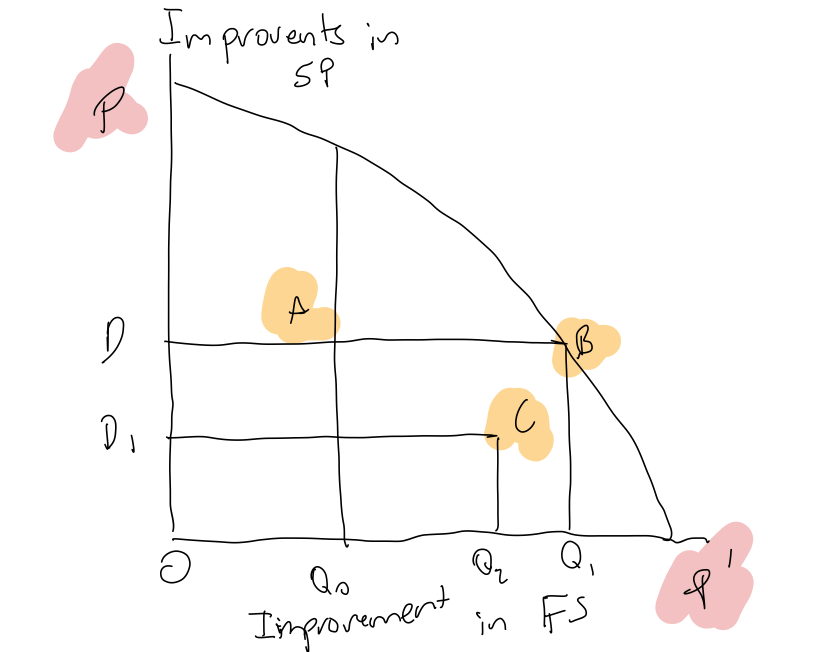
\includegraphics[width=11.58in]{images/fig1} 

}

\caption{Production possibilities frontier}\label{fig:fig1}
\end{figure}

In practice, CEA \textbf{relaxes the constraint on available resources}. Because the focus of the evaluation is not a fixed resource pool, but a specific programme making demands on resources, the comparison of the programme under evaluation with an existing programme (e.g., services aimed at improving FS) must consider not only the inter-programme differences in outputs (incremental benefits), but also the inter-programme differences in resources used (incremental costs).

\citet{weinstein1977foundations} state that: \emph{``the criterion for cost-effectiveness is the ratio of the net increase of health-care costs to the net effectiveness. The lower the value of this ratio, the higher the priority in terms of maximizing benefits derived from a given health expenditure''}. Issue is that applying a ratio does nod lead to the maximization of benefits from a fixed resource pool (movement from A to C in Figure). \textbf{The real problem of the application of CEA is the failure to adhere strictly to the notion of opportunity cost in the measurement of the (incremental) cost of a programme.} The existing programme represents a true opportunity cost for the entire resource requirements of the new programme, even though it does not absorb this level of resources.

\hypertarget{cost-effectiveness-in-practice}{%
\subsection{Cost-effectiveness in practice}\label{cost-effectiveness-in-practice}}

As mentioned before, CEA include both costs and effects, which are represented graphically in a plane:

\begin{figure}

{\centering 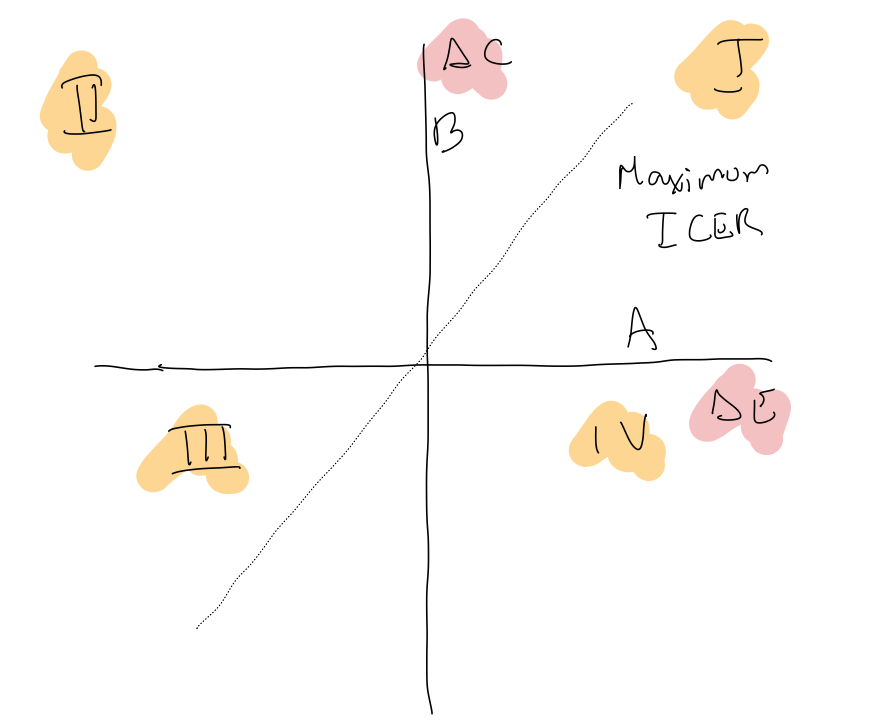
\includegraphics[width=12.31in]{images/fig2} 

}

\caption{Incremental CE plane}\label{fig:fig2}
\end{figure}

\textbf{Questions}

\begin{enumerate}
\def\labelenumi{\arabic{enumi}.}
\tightlist
\item
  Describe the plane.
\item
  What is the willingness-to-pay in this plane?
\item
  What type of uncertainties are encountered in this plane?
\end{enumerate}

Why incremental? We can see it using the example from \citet{gray2011applied} applied to mutually exclusive options (see Figure \ref{fig:fig3}):

\begin{itemize}
\tightlist
\item
  Diet and excercise (C): Reference
\item
  Metformin (A): \$500k/250 life-years
\item
  New drug (B): \$2500k/300 life-years
\end{itemize}

\begin{figure}

{\centering 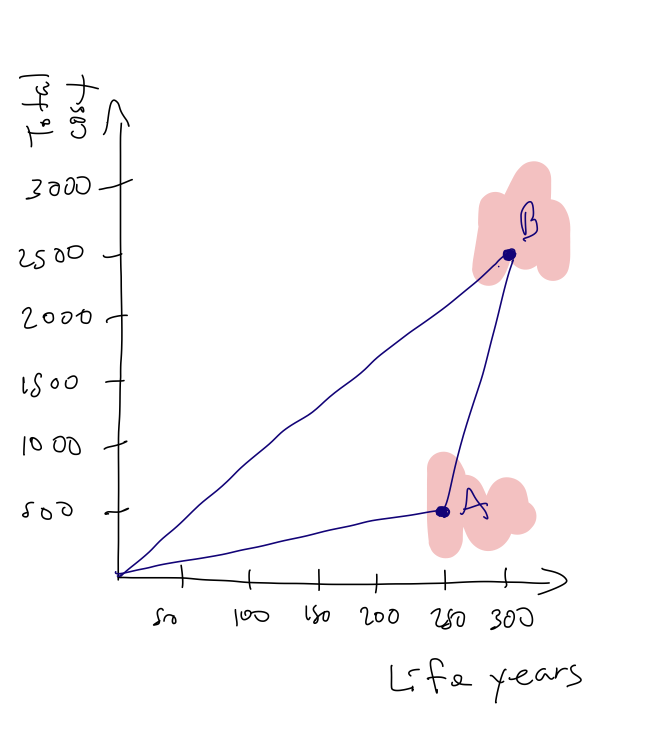
\includegraphics[width=9.25in]{images/fig3} 

}

\caption{Average and incremental cost-effectivenessr}\label{fig:fig3}
\end{figure}

Clearly, as this example shows, it is quite misleading to calculate average cost-effectiveness ratios, as they ignore the alternatives available.

\textbf{Questions}

\begin{enumerate}
\def\labelenumi{\arabic{enumi}.}
\tightlist
\item
  What is the difference between average cost-effectiveness ratios vs incremental?
\end{enumerate}

The idea of CEA is to maximize health benefits with the available resources, which in terms of the CE plane represents pushing as far to the right as possible while moving up the vertical axis as little as possible. The next example from \citet{gray2011applied} shows the ideas behind \textbf{cost-effectivness frontier, dominance, extended dominance} (Table \ref{tab:table2}).

\begin{table}

\caption{\label{tab:table2}Calculating incremental cost-effectiveness}
\centering
\begin{tabular}[t]{l|r|r|r|r|r}
\hline
Option & Cost & QALYs & Incremental cost & Incremental QALY & ICER\\
\hline
A & 0 &  &  &  & \\
\hline
B & 10,000 & 0.40 & 10,000 & 0.40 & 25,000\\
\hline
C & 22,000 & 0.55 & 12,000 & 0.15 & 80,000\\
\hline
D & 25,000 & 0.50 & 3,000 & -0.05 & -60,000\\
\hline
E & 40,000 & 1.00 & 15,000 & 0.50 & 30,000\\
\hline
\end{tabular}
\end{table}

Once we have the ICERs for different independent programmes. How can we maximize health gains with this information? Note that now we are comparing different programmes as opposed to mutually exclusive options. Let's work in the next example:

\begin{table}

\caption{\label{tab:table3}Using cost-effectiveness to maximize health gain}
\centering
\begin{tabular}[t]{l|r|r|r}
\hline
Intervention & Incremental cost (per k) & Incremental QALYs & ICER\\
\hline
1 & 1,300 & 165 & 7,879\\
\hline
2 & 600 & 28 & 21,429\\
\hline
3 & 750 & 110 & 6,818\\
\hline
4 & 750 & 13 & 57,692\\
\hline
5 & 2,200 & 75 & 29,333\\
\hline
6 & 400 & 85 & 4,706\\
\hline
Total & 6,000 & 476 & \\
\hline
\end{tabular}
\end{table}

Finally, we can ask ourselves. What is the maximum value of the incremental cost-effectivess ratio (\(\lambda\))?

\begin{itemize}
\item
  Rule-based approaches - Adopting arbitrary thresholds. For example, \citet{laupacis1992attractive} adopted identical cut-off points of CAN\$20,000 per QALY gained, up to which level they considered that there would be strong grounds for adoption, and CAN\$100,000 per QALY gained, above which they considered that evidence for adoption was weak. An alternative approach is to use the country's gross domestic product (GDP) per capita. \citet{williams2004could} advanced one line of reasoning in support of this, arguing that each
  person has an entitlement to a `fair share' of the country's wealth.
\item
  League table approach - If we had full information on the ICERs of all available interventions, it would be possible to rank them by ICER. See the example in Table \ref{tab:table2}.
\end{itemize}

What are the issues with these approaches?

\begin{enumerate}
\def\labelenumi{\arabic{enumi}.}
\tightlist
\item
  \(\lambda\) is a function of the budget. Therefore it is constantly changing
\item
  The dynamic nature of \(\lambda\). As new programs are funded and others replaced, the identification of the last program funded changes.
\end{enumerate}

\hypertarget{conclusions}{%
\subsection{Conclusions}\label{conclusions}}

\begin{itemize}
\item
  Irrespective of whether the problem face by decision-makers is simple (maximizing health gains from available resources) or complex (subject to considerations of equity, accessibility, etc.), if it is not to be considered in the context of a resource constraint there is little use for economics in the way the problem is considered.
\item
  Other approaches have been considered, such as methods in linear programming, which is consistent with the objective of CEA.
\end{itemize}

\[
\max_{x_i,\dots,x_n}\sum_{i=1}^n x_iE_i\\
\text{s.t.}\ \ \ \ \ \sum_{i=1}^n x_ic_i\leq C
\]

where \(x_i\) is the health intervention presented as a binary outcome (1 or 0), \(E_i\) is the present value of the health benefits (measured using QALYs) generated by programme over the planning period, and \(c_i\) is the present value of the cost of providing programme \(i\) over the planning period.

\hypertarget{decision-modelling}{%
\section{Decision modelling}\label{decision-modelling}}

HTA is undertaken in order to inform decision-making regarding the appropriate use of particular healthcare programs and interventions, and involves the synthesis of a range of evidence. Broadly speaking, this implies two important components of this process:

\begin{enumerate}
\def\labelenumi{\arabic{enumi}.}
\item
  Gathering evidence for the disease and technology of concern from a range of primary studies. This includes effectiveness, costs, epidemiology, natural history of the disease, quality of life, etc.
\item
  Synthesizing the evidence found in the first component in order to inform policy and decision-making.
\end{enumerate}

Because of the nature of these two components, decision-analytic modelling has played an important role in HTA. This is because it represents an explicit approach to synthesizing currently available evidence regarding the effectiveness and costs of alternative (mutually exclusive) healthcare strategies \citep{philips2006good}. Therefore one of the main objectives of decision-analytic modelling is to address the relationship between the effectiveness and costs of alternative healthcare strategies in order to assess relative cost-effectiveness (CE) and to determine which options should be adopted given existing information \citep{philips2006good}. Consequently, modelling in the context of HTA is a typical problem of decision-making under uncertainty.

Traditionally randomised controlled trials (RCTs) have been a key component of many HTA process. This is because randomsation protects against selection bias and confounding. Nevertheless, the information produced by RCTs can be limited with respect to evaluating health care as delivered in the real world. This can be because:

\begin{enumerate}
\def\labelenumi{\arabic{enumi}.}
\tightlist
\item
  Not all interventions to be compared are included in the trial.
\item
  Not enough follow-up.
\item
  Not enough flexibility (controlled trial).
\item
  Small sample sizes.
\item
  Patients in trial are not representative to the target population.
\end{enumerate}

Consequently, it is advised that HTA submissions incorporate information from as many sources as possible to address some of these problems \citep{sculpher2006whither}. As mentioned before, decision analytical models allow for the synthesis of information across multiple sources and for the comparison of multiple options that might not have been included as part of an RCT.

Briefly, \citet{dahabreh2016guidance} consider some potential goals of modelling in a health-care context:

\begin{itemize}
\tightlist
\item
  To structure investigators' thinking and to facilitate the communication of data, assumptions, and results.
\item
  To synthesize data from disparate sources.
\item
  To make predictions.
\item
  To support causal explanations.
\item
  To inform decision making.
\end{itemize}

Moreover, they also distinguish different stages for the development of a decision analytic model

\begin{enumerate}
\def\labelenumi{\arabic{enumi}.}
\tightlist
\item
  Define a question
\item
  Decide on the type of decision model most appropriate
\item
  Conceptualize the model (and its mathematical structure).
\item
  Gather all the evidence required for the model and synthesize it.
\item
  Implement and run the model.
\item
  Assess the model.
\end{enumerate}

The development of models, especially those trying to explain complex phenoma and informing difficult decisions, is a demanding task. Choosing between alternative modeling approaches can be difficult because the correct choice would not be obvious at early stages in developing a decision analytical model. In general, modelling is most useful when data have limitations (e.g.~non-randomised evidence, sparse evidence, etc.), when the research question is complex and when choices are preference laden \citep{dahabreh2016guidance}. Another important aspect when choosing between modelling approaches is whether the model in question is likely to show results that the intended audience will consider credible and useful. Multiple iterations are typically needed between the key activities outlined previously because at each activity the need for changes at earlier stages may become evident.

\hypertarget{importance-of-decision-analytic-models-in-hta}{%
\subsection{Importance of decision-analytic models in HTA}\label{importance-of-decision-analytic-models-in-hta}}

When doing a cost-effectiveness analysis in the context of HTA, one usually starts conceptualizing the model that will help answer the research question. But what is a model? A model a simplified representation of reality \citep{roberts2012conceptualizing}, where inputs from different sources inform it and its purpose, in the context of HTA, is to inform medical decisions and health-related resource allocation questions \citep{roberts2012conceptualizing}.

Methods for the conduct of decision-analytic modelling have continued evolving to address the ever-increasing information needs of decision makers. The complexity and continued advances of the relevant methods have spurred the publication of recommendation statements on ``best practices'' for modeling in the context of HTA \citep{roberts2012conceptualizing, briggs2012model}. Some of these modelling techniques \citep{caro2012modeling} include:

\begin{itemize}
\tightlist
\item
  Decision-tree models.
\item
  State-transition models.
\item
  Micro-simulation models.
\item
  Discrete event simulation (DES) models.
\item
  Dynamic transmission models.
\end{itemize}

\hypertarget{excercises-1}{%
\section{Excercises}\label{excercises-1}}

\begin{enumerate}
\def\labelenumi{\arabic{enumi}.}
\tightlist
\item
  Question 1 and 2 from Chapter 2 in \emph{Applied methods of cost-effectiveness analysis in healthcare }.
\item
  Read the articles in our google classroom.
\end{enumerate}

\hypertarget{tree}{%
\chapter{Good practices in decision modelling and decion-tree models}\label{tree}}

\hypertarget{pre-session-readings-2}{%
\section{Pre-session readings}\label{pre-session-readings-2}}

\textbf{Good practices}

\emph{Roberts, M., Russell, L. B., Paltiel, A. D., Chambers, M., McEwan, P., \& Krahn, M. (2012). Conceptualizing a model: a report of the ISPOR-SMDM modeling good research practices task force--2. Medical Decision Making, 32(5), 678-689.}

\textbf{Decision-tree models}

\emph{Tarride, J. E., Blackhouse, G., Bischof, M., McCarron, E. C., Lim, M., Ferrusi, I. L., \ldots{} \& Goeree, R. (2009). Approaches for economic evaluations of health care technologies. Journal of the American College of Radiology, 6(5), 307-316.}

\emph{Briggs, A., Sculpher, M., \& Claxton, K. (2006). Decision modelling for health economic evaluation. Oxford University Press.} Chapter 2. Sections 2.2 and 2.3.1.

\emph{Gray, A. M., Clarke, P. M., Wolstenholme, J. L., \& Wordsworth, S. (2011). Applied methods of cost-effectiveness analysis in healthcare (Vol. 3). Oxford University Press.} Chapter 8. Sections 8.5 and 8.6.

\hypertarget{introduction-to-r}{%
\chapter*{Introduction to R}\label{introduction-to-r}}
\addcontentsline{toc}{chapter}{Introduction to R}

The goal of this tutorial is to orient the learner to R Studio and the R programming language.

Please complete the following:

\begin{enumerate}
\def\labelenumi{\arabic{enumi}.}
\tightlist
\item
  Create a folder somewhere you can easily find it (e.g., on your desktop) called `R Course'.
\item
  Open R Studio
\item
  Session -\textgreater{} Set Working Directory -\textgreater{} to source file location
\end{enumerate}

\hypertarget{outline}{%
\section*{Outline}\label{outline}}
\addcontentsline{toc}{section}{Outline}

\begin{enumerate}
\def\labelenumi{\arabic{enumi}.}
\tightlist
\item
  Read in the `babies' data set
\item
  Basic data manipulation
\item
  Functions
\item
  Saving and viewing results
\end{enumerate}

\hypertarget{babies-dataset}{%
\section*{Babies Dataset}\label{babies-dataset}}
\addcontentsline{toc}{section}{Babies Dataset}

The \texttt{babies} dataset will be used throughout this session to illustrate basic R concepts.

The dataset is a collection of variables taken for each new mother in a Child and Health Development Study. It has 1,236 observations on male live births for the following 23 variables.

Variables in data file

\begin{verbatim}
id            identification number
date          birth date as character string (mon-dd-yyyy)
ddate         day of birth
mdate         month of birth
ydate         year of birth
gestation     length of gestation in days
wt            birth weight in ounces (999 unknown)
parity        total number of previous pregnancies 
              including fetal deaths and still births
age           mother's age in years at end of pregnancy
                999=unknown
ed            mother's education 
                 0=less than 8th grade
                 1=8th-12th grade - did not graduate
                 2=HS graduate???no other schooling
                 3=HS+trade
                 4=HS+some college
                 5=College graduate,
                 6=Trade school HS unclear
                 9=unknown
ht            mother's height in inches to the last completed inch 
                 999=unknown
wt1           mother prepregnancy wt in pounds
                 999=unknown
dage          father's age, coding same as mother's age.
ded           father's education, coding same as mother's education.
dht           father's height, coding same as for mother's height
dwt           father's weight coding same as for mother's weight
inc           family yearly income in $2500 increments
                 0=under 2500
                 1=2500-4999
                 ..., 
                 8= 12,500-14,999
                 9=15000+
                 998=unknown
                 999=not asked
smoke         does mother smoke? 
                 0=never
                 1=smokes now
                 2=until current pregnancy
                 3=once did, not now
                 9=unknown
time          If mother quit smoking, how long ago? 
                 0=never smoked
                 1=still smokes
                 2=during current preg
                 3=within 1 yr
                 4=1 to 2 years ago
                 5=2 to 3 years ago
                 6=3 to 4 years ago
                 7=5 to 9 years ago 
                 8=10+years ago
                 9=quit and don't know,
                 998=unknown
                 999=not asked
number        number of cigs smoked per day for past and current smokers 
                 0=never
                 1=1-4
                 2=5-9
                 3=10-14
                 4=15-19
                 5=20-29
                 6=30-39
                 7=40-60
                 8=60+
                 9=smoke but don't know
                 998=unknown
                 999=not asked
race          mother's race 
marital       marital status of mother
drace         father's race, coding same as mother's race
\end{verbatim}

\hypertarget{loading-babies-dataset}{%
\subsection*{Loading babies dataset}\label{loading-babies-dataset}}
\addcontentsline{toc}{subsection}{Loading babies dataset}

We can can load the data from our working directory as shown below. It is a .csv file, so can be read in with \texttt{read.csv}. specifying that

\begin{itemize}
\tightlist
\item
  the file has a ``header'' row (\texttt{header=T}) with variable names
\item
  values are separated by commas.\\
\item
  values of '`, '998' or `999' represent missing data
\end{itemize}

We need to be confident that 998 and 999 are not legitimate values for any variables, so that R does not interpret legitimate values as missing. We will not distinguish between `unknown' and `not asked' in the data, so the code below will read two consecutive commas (```), 998, and 999 as missing values. We will have to deal separately with the values '9' that mean a value is missing.

\begin{Shaded}
\begin{Highlighting}[]
\NormalTok{babies }\OtherTok{\textless{}{-}} \FunctionTok{read.csv}\NormalTok{(}\StringTok{\textquotesingle{}babies.csv\textquotesingle{}}\NormalTok{,}\AttributeTok{header=}\NormalTok{T, }\AttributeTok{sep=}\StringTok{","}\NormalTok{, }
                     \AttributeTok{na.strings=}\FunctionTok{c}\NormalTok{(}\StringTok{""}\NormalTok{, }\StringTok{"998"}\NormalTok{, }\StringTok{"999"}\NormalTok{))}
\end{Highlighting}
\end{Shaded}

\hypertarget{data-manipulation}{%
\subsection*{Data manipulation}\label{data-manipulation}}
\addcontentsline{toc}{subsection}{Data manipulation}

What are the dimensions of the data set?

\begin{Shaded}
\begin{Highlighting}[]
\FunctionTok{dim}\NormalTok{(babies)}
\end{Highlighting}
\end{Shaded}

{[}1{]} 1236 23

What are the names of the variables?

\begin{Shaded}
\begin{Highlighting}[]
\FunctionTok{names}\NormalTok{(babies)}
\end{Highlighting}
\end{Shaded}

\begin{verbatim}
##  [1] "id"        "date"      "gestation" "wt"        "parity"    "age"      
##  [7] "ed"        "ht"        "wt1"       "dage"      "ded"       "dht"      
## [13] "dwt"       "inc"       "smoke"     "time"      "number"    "race"     
## [19] "marital"   "drace"     "ddate"     "mdate"     "ydate"
\end{verbatim}

\begin{Shaded}
\begin{Highlighting}[]
\CommentTok{\#head(babies)}
\CommentTok{\#tail(babies)}
\end{Highlighting}
\end{Shaded}

Isolating variables

\begin{Shaded}
\begin{Highlighting}[]
\CommentTok{\# babies$id}
\CommentTok{\# babies[, 1]}
\CommentTok{\# babies[, \textquotesingle{}id\textquotesingle{}]}
\CommentTok{\# babies[1:10, c(\textquotesingle{}id\textquotesingle{}, \textquotesingle{}date\textquotesingle{}, \textquotesingle{}gestation\textquotesingle{})]}
\end{Highlighting}
\end{Shaded}

Assignment and subsetting

\begin{Shaded}
\begin{Highlighting}[]
\NormalTok{under}\FloatTok{.30}\OtherTok{\textless{}{-}}\NormalTok{ babies}\SpecialCharTok{$}\NormalTok{age}\SpecialCharTok{\textless{}}\DecValTok{30}
\NormalTok{b}\OtherTok{\textless{}{-}}\NormalTok{ babies[under}\FloatTok{.30}\NormalTok{, ]}
\FunctionTok{summary}\NormalTok{(b}\SpecialCharTok{$}\NormalTok{age)}
\end{Highlighting}
\end{Shaded}

\begin{verbatim}
##    Min. 1st Qu.  Median    Mean 3rd Qu.    Max.    NA's 
##   15.00   22.00   24.00   24.03   27.00   29.00       2
\end{verbatim}

\begin{Shaded}
\begin{Highlighting}[]
\NormalTok{b}\OtherTok{\textless{}{-}}\NormalTok{ babies[}\FunctionTok{which}\NormalTok{(under}\FloatTok{.30}\NormalTok{), ]}
\FunctionTok{summary}\NormalTok{(b}\SpecialCharTok{$}\NormalTok{age)}
\end{Highlighting}
\end{Shaded}

\begin{verbatim}
##    Min. 1st Qu.  Median    Mean 3rd Qu.    Max. 
##   15.00   22.00   24.00   24.03   27.00   29.00
\end{verbatim}

\hypertarget{exercises-1}{%
\subsubsection*{Exercises (1)}\label{exercises-1}}
\addcontentsline{toc}{subsubsection}{Exercises (1)}

\begin{enumerate}
\def\labelenumi{\arabic{enumi}.}
\item
  Create a new data set consisting of only the rows where the father's age is 40 or over (use `\textgreater=')
\item
  Include only the mother's age, father's age and marital status in the new dataset
\item
  Display the dimensions of this data set in the console.
\item
  Locate the new dataset in th Global Environment and view it
\end{enumerate}

NB: Be sure that you have handled missing father's ages properly

\hypertarget{exercises-1-solutions}{%
\paragraph*{Exercises (1) solutions}\label{exercises-1-solutions}}
\addcontentsline{toc}{paragraph}{Exercises (1) solutions}

\hypertarget{creating-some-new-variables}{%
\subsection*{Creating some new variables}\label{creating-some-new-variables}}
\addcontentsline{toc}{subsection}{Creating some new variables}

A baby weight more than 4kg is defined as macrosomia. We can create this variable (converting ounces to kg) as:

\begin{Shaded}
\begin{Highlighting}[]
\NormalTok{babies}\SpecialCharTok{$}\NormalTok{wtKg }\OtherTok{\textless{}{-}}\NormalTok{ babies}\SpecialCharTok{$}\NormalTok{wt}\SpecialCharTok{/}\NormalTok{(}\DecValTok{16}\SpecialCharTok{*}\FloatTok{2.2}\NormalTok{)}
\NormalTok{babies}\SpecialCharTok{$}\NormalTok{macrosomia }\OtherTok{\textless{}{-}}\NormalTok{ babies}\SpecialCharTok{$}\NormalTok{wtKg }\SpecialCharTok{\textgreater{}} \DecValTok{4}
\end{Highlighting}
\end{Shaded}

A baby weighing less than 2.5kg is defined as ``small''. We can create this variable as:

\begin{Shaded}
\begin{Highlighting}[]
\NormalTok{babies}\SpecialCharTok{$}\NormalTok{smallBaby }\OtherTok{\textless{}{-}}\NormalTok{ babies}\SpecialCharTok{$}\NormalTok{wtKg }\SpecialCharTok{\textless{}} \FloatTok{2.5}
\end{Highlighting}
\end{Shaded}

We can make a single character variable with three categories of weight:

\begin{Shaded}
\begin{Highlighting}[]
\NormalTok{babies}\SpecialCharTok{$}\NormalTok{birthWeightCat }\OtherTok{\textless{}{-}} \FunctionTok{ifelse}\NormalTok{(babies}\SpecialCharTok{$}\NormalTok{wtKg }\SpecialCharTok{\textless{}} \FloatTok{2.5}\NormalTok{, }\StringTok{"small"}\NormalTok{,}
                                \FunctionTok{ifelse}\NormalTok{(babies}\SpecialCharTok{$}\NormalTok{wtKg }\SpecialCharTok{\textgreater{}} \DecValTok{4}\NormalTok{, }\StringTok{"large"}\NormalTok{,}\StringTok{"normal"}\NormalTok{))}
\end{Highlighting}
\end{Shaded}

Notice that when we tabulate these, they appear in alphabetical order.

\begin{Shaded}
\begin{Highlighting}[]
\FunctionTok{table}\NormalTok{(babies}\SpecialCharTok{$}\NormalTok{birthWeightCat)}
\end{Highlighting}
\end{Shaded}

\begin{verbatim}
## 
##  large normal  small 
##    145   1033     58
\end{verbatim}

To impose an order, we can convert to a factor and specify the order:

\begin{Shaded}
\begin{Highlighting}[]
\NormalTok{babies}\SpecialCharTok{$}\NormalTok{birthWeightCat }\OtherTok{\textless{}{-}} \FunctionTok{factor}\NormalTok{(babies}\SpecialCharTok{$}\NormalTok{birthWeightCat, }
                                  \AttributeTok{levels=}\FunctionTok{c}\NormalTok{(}\StringTok{"small"}\NormalTok{,}\StringTok{"normal"}\NormalTok{,}\StringTok{"large"}\NormalTok{),}
                                  \AttributeTok{labels=}\FunctionTok{c}\NormalTok{(}\StringTok{"Small baby"}\NormalTok{,}\StringTok{"Normal weight baby"}\NormalTok{,}\StringTok{"Large baby"}\NormalTok{))}
\FunctionTok{table}\NormalTok{(babies}\SpecialCharTok{$}\NormalTok{birthWeightCat)                                }
\end{Highlighting}
\end{Shaded}

\begin{verbatim}
## 
##         Small baby Normal weight baby         Large baby 
##                 58               1033                145
\end{verbatim}

A baby born before 37 completed weeks of pregnancy is defined as preterm. We can create this logical variable as:

\begin{Shaded}
\begin{Highlighting}[]
\NormalTok{babies}\SpecialCharTok{$}\NormalTok{preterm }\OtherTok{\textless{}{-}}\NormalTok{ babies}\SpecialCharTok{$}\NormalTok{gestation }\SpecialCharTok{\textless{}} \DecValTok{37}\SpecialCharTok{*}\DecValTok{7}
\FunctionTok{table}\NormalTok{(babies}\SpecialCharTok{$}\NormalTok{preterm)}
\end{Highlighting}
\end{Shaded}

\begin{verbatim}
## 
## FALSE  TRUE 
##  1126    97
\end{verbatim}

This is just a logical variable (\texttt{TRUE/FALSE} or \texttt{T/F}) so we need to make a factor to have it appear more user-friendly:

\begin{Shaded}
\begin{Highlighting}[]
\NormalTok{babies}\SpecialCharTok{$}\NormalTok{whenBorn }\OtherTok{\textless{}{-}} \FunctionTok{factor}\NormalTok{(babies}\SpecialCharTok{$}\NormalTok{preterm, }
                          \AttributeTok{levels=}\FunctionTok{c}\NormalTok{(}\ConstantTok{TRUE}\NormalTok{,}\ConstantTok{FALSE}\NormalTok{), }
                          \AttributeTok{labels=}\FunctionTok{c}\NormalTok{(}\StringTok{"Preterm"}\NormalTok{,}\StringTok{"Full{-}term"}\NormalTok{))}
\end{Highlighting}
\end{Shaded}

We can make a binary variable for the mother's and father's races:

\begin{Shaded}
\begin{Highlighting}[]
\NormalTok{babies}\SpecialCharTok{$}\NormalTok{whiteRace }\OtherTok{\textless{}{-}} \FunctionTok{ifelse}\NormalTok{(babies}\SpecialCharTok{$}\NormalTok{race}\SpecialCharTok{==}\StringTok{"white"}\NormalTok{,}\StringTok{"white"}\NormalTok{,}\StringTok{"other"}\NormalTok{)}
\NormalTok{babies}\SpecialCharTok{$}\NormalTok{dwhiteRace }\OtherTok{\textless{}{-}} \FunctionTok{ifelse}\NormalTok{(babies}\SpecialCharTok{$}\NormalTok{drace}\SpecialCharTok{==}\StringTok{"white"}\NormalTok{,}\StringTok{"white"}\NormalTok{,}\StringTok{"other"}\NormalTok{)}
\end{Highlighting}
\end{Shaded}

\hypertarget{exercises-2}{%
\subsubsection*{Exercises (2)}\label{exercises-2}}
\addcontentsline{toc}{subsubsection}{Exercises (2)}

\begin{enumerate}
\def\labelenumi{\arabic{enumi}.}
\tightlist
\item
  Starting with the numeric variable \texttt{smoke}, in the babies dataset, create a new variable \texttt{smokeCat} in the data set that has three levels: \texttt{never\ smoker}, \texttt{past\ smoker},\texttt{current\ smoker}. Use the \texttt{factor} function and ensure that the levels appear in that order.
\item
  Tabulate the numerical variable against the new one to make sure you have not made an error.
\item
  Make a binary variable in the babies dataset \texttt{smokeNow} that is `Yes' when the mother smokes and `No' otherwise (i.e., it is not yes (1) or it is missing (9).)
\item
  {[}optional{]} Make a factor variable \texttt{eduCat} from the mother's education variable \texttt{ed} using the information at the top if this file about the meaning of 1,2,3,\ldots{}
\end{enumerate}

\hypertarget{exercises-2-solutions}{%
\paragraph*{Exercises (2) solutions}\label{exercises-2-solutions}}
\addcontentsline{toc}{paragraph}{Exercises (2) solutions}

\begin{enumerate}
\def\labelenumi{\arabic{enumi}.}
\item
  Make the two variables:
\item
  Check the coding was correct
\item
  Make a binary variable
\item
  {[}optional{]} make the education variable and check it
\end{enumerate}

\hypertarget{functions}{%
\section*{Functions}\label{functions}}
\addcontentsline{toc}{section}{Functions}

Two types:

\begin{enumerate}
\def\labelenumi{\arabic{enumi}.}
\tightlist
\item
  Built in functions
\item
  User defined functions
\end{enumerate}

\hypertarget{built-in-functions}{%
\subsection*{Built in Functions}\label{built-in-functions}}
\addcontentsline{toc}{subsection}{Built in Functions}

When you open R, there are many functions available to you: Here, we will review a few useful built in functions.

If you need help using a function, execute ? followed by the function name, with or without the parentheses.

\begin{verbatim}
? table
\end{verbatim}

The following functions are widely used in descriptive statistics

\hypertarget{table-prop.table}{%
\subsubsection*{table(), prop.table()}\label{table-prop.table}}
\addcontentsline{toc}{subsubsection}{table(), prop.table()}

\begin{Shaded}
\begin{Highlighting}[]
\NormalTok{t}\OtherTok{\textless{}{-}} \FunctionTok{with}\NormalTok{(babies, }\FunctionTok{table}\NormalTok{(marital))}
\NormalTok{t}
\end{Highlighting}
\end{Shaded}

\begin{verbatim}
## marital
##          divorced legally separated           married     never married 
##                 5                15              1208                 6 
##           unknown 
##                 2
\end{verbatim}

\begin{Shaded}
\begin{Highlighting}[]
\NormalTok{p}\OtherTok{\textless{}{-}} \FunctionTok{prop.table}\NormalTok{(t)}
\NormalTok{p}
\end{Highlighting}
\end{Shaded}

\begin{verbatim}
## marital
##          divorced legally separated           married     never married 
##       0.004045307       0.012135922       0.977346278       0.004854369 
##           unknown 
##       0.001618123
\end{verbatim}

\begin{Shaded}
\begin{Highlighting}[]
\NormalTok{p}\SpecialCharTok{*}\DecValTok{100}
\end{Highlighting}
\end{Shaded}

\begin{verbatim}
## marital
##          divorced legally separated           married     never married 
##         0.4045307         1.2135922        97.7346278         0.4854369 
##           unknown 
##         0.1618123
\end{verbatim}

\hypertarget{ifelse}{%
\subsubsection*{ifelse()}\label{ifelse}}
\addcontentsline{toc}{subsubsection}{ifelse()}

\begin{Shaded}
\begin{Highlighting}[]
\NormalTok{babies}\SpecialCharTok{$}\NormalTok{first.preg}\OtherTok{\textless{}{-}} \FunctionTok{with}\NormalTok{(babies, }\FunctionTok{ifelse}\NormalTok{(parity}\SpecialCharTok{==}\DecValTok{0}\NormalTok{, }\StringTok{\textquotesingle{}first\textquotesingle{}}\NormalTok{,}\StringTok{\textquotesingle{}not first\textquotesingle{}}\NormalTok{))}
\FunctionTok{table}\NormalTok{(babies}\SpecialCharTok{$}\NormalTok{first.preg)}
\end{Highlighting}
\end{Shaded}

\begin{verbatim}
## 
##     first not first 
##       315       921
\end{verbatim}

\hypertarget{summary-mean-median-sd-quantile}{%
\subsubsection*{summary(), mean(), median(), sd(), quantile()}\label{summary-mean-median-sd-quantile}}
\addcontentsline{toc}{subsubsection}{summary(), mean(), median(), sd(), quantile()}

\begin{Shaded}
\begin{Highlighting}[]
\FunctionTok{summary}\NormalTok{(babies)}
\end{Highlighting}
\end{Shaded}

\begin{verbatim}
##        id           date             gestation           wt       
##  Min.   :  15   Length:1236        Min.   :148.0   Min.   : 55.0  
##  1st Qu.:5286   Class :character   1st Qu.:272.0   1st Qu.:108.8  
##  Median :6730   Mode  :character   Median :280.0   Median :120.0  
##  Mean   :6001                      Mean   :279.3   Mean   :119.6  
##  3rd Qu.:7583                      3rd Qu.:288.0   3rd Qu.:131.0  
##  Max.   :9263                      Max.   :353.0   Max.   :176.0  
##                                    NA's   :13                     
##      parity            age              ed              ht       
##  Min.   : 0.000   Min.   :15.00   Min.   :0.000   Min.   :53.00  
##  1st Qu.: 0.000   1st Qu.:23.00   1st Qu.:2.000   1st Qu.:62.00  
##  Median : 1.000   Median :26.00   Median :2.000   Median :64.00  
##  Mean   : 1.932   Mean   :27.26   Mean   :2.916   Mean   :64.05  
##  3rd Qu.: 3.000   3rd Qu.:31.00   3rd Qu.:4.000   3rd Qu.:66.00  
##  Max.   :13.000   Max.   :45.00   Max.   :9.000   Max.   :72.00  
##                   NA's   :2                       NA's   :22     
##       wt1             dage            ded             dht            dwt       
##  Min.   : 87.0   Min.   :18.00   Min.   :0.000   Min.   :60.0   Min.   :110.0  
##  1st Qu.:114.8   1st Qu.:25.00   1st Qu.:2.000   1st Qu.:68.0   1st Qu.:155.0  
##  Median :125.0   Median :29.00   Median :4.000   Median :71.0   Median :170.0  
##  Mean   :128.6   Mean   :30.35   Mean   :3.189   Mean   :70.2   Mean   :171.2  
##  3rd Qu.:139.0   3rd Qu.:34.00   3rd Qu.:5.000   3rd Qu.:72.0   3rd Qu.:185.0  
##  Max.   :250.0   Max.   :62.00   Max.   :9.000   Max.   :78.0   Max.   :260.0  
##  NA's   :36      NA's   :7                       NA's   :492    NA's   :499    
##       inc            smoke             time            number     
##  Min.   :0.000   Min.   :0.0000   Min.   :0.0000   Min.   :0.000  
##  1st Qu.:2.000   1st Qu.:0.0000   1st Qu.:0.0000   1st Qu.:0.000  
##  Median :3.000   Median :1.0000   Median :1.0000   Median :1.000  
##  Mean   :3.701   Mean   :0.8681   Mean   :0.9625   Mean   :1.825  
##  3rd Qu.:5.000   3rd Qu.:1.0000   3rd Qu.:1.0000   3rd Qu.:3.000  
##  Max.   :9.000   Max.   :9.0000   Max.   :9.0000   Max.   :9.000  
##  NA's   :124                      NA's   :10       NA's   :10     
##      race             marital             drace               ddate      
##  Length:1236        Length:1236        Length:1236        Min.   : 1.00  
##  Class :character   Class :character   Class :character   1st Qu.: 8.00  
##  Mode  :character   Mode  :character   Mode  :character   Median :15.00  
##                                                           Mean   :15.37  
##                                                           3rd Qu.:23.00  
##                                                           Max.   :31.00  
##                                                                          
##      mdate            ydate           wtKg       macrosomia     
##  Min.   : 1.000   Min.   :1961   Min.   :1.562   Mode :logical  
##  1st Qu.: 4.000   1st Qu.:1961   1st Qu.:3.089   FALSE:1091     
##  Median : 7.000   Median :1962   Median :3.409   TRUE :145      
##  Mean   : 6.617   Mean   :1962   Mean   :3.397                  
##  3rd Qu.: 9.000   3rd Qu.:1962   3rd Qu.:3.722                  
##  Max.   :12.000   Max.   :1962   Max.   :5.000                  
##                                                                 
##  smallBaby                  birthWeightCat  preterm             whenBorn   
##  Mode :logical   Small baby        :  58   Mode :logical   Preterm  :  97  
##  FALSE:1178      Normal weight baby:1033   FALSE:1126      Full-term:1126  
##  TRUE :58        Large baby        : 145   TRUE :97        NA's     :  13  
##                                            NA's :13                        
##                                                                            
##                                                                            
##                                                                            
##   whiteRace          dwhiteRace                  smokeCat     smokeNow        
##  Length:1236        Length:1236        Never smoker  :544   Length:1236       
##  Class :character   Class :character   Past smoker   :198   Class :character  
##  Mode  :character   Mode  :character   Current smoker:484   Mode  :character  
##                                        NA's          : 10                     
##                                                                               
##                                                                               
##                                                                               
##               eduCat     first.preg       
##  HS graduate     :444   Length:1236       
##  HS+some college :298   Class :character  
##  College graduate:219   Mode  :character  
##  8th-12th grade  :183                     
##  HS+trade        : 65                     
##  (Other)         : 26                     
##  NA's            :  1
\end{verbatim}

\begin{Shaded}
\begin{Highlighting}[]
\NormalTok{gestAge}\OtherTok{\textless{}{-}}\NormalTok{ babies}\SpecialCharTok{$}\NormalTok{gestation}
\FunctionTok{mean}\NormalTok{(gestAge)}
\end{Highlighting}
\end{Shaded}

\begin{verbatim}
## [1] NA
\end{verbatim}

\begin{Shaded}
\begin{Highlighting}[]
\FunctionTok{mean}\NormalTok{(gestAge, }\AttributeTok{na.rm=}\NormalTok{T)}
\end{Highlighting}
\end{Shaded}

\begin{verbatim}
## [1] 279.3385
\end{verbatim}

\begin{Shaded}
\begin{Highlighting}[]
\NormalTok{gestAge}\OtherTok{\textless{}{-}}\NormalTok{ gestAge[}\FunctionTok{complete.cases}\NormalTok{(gestAge)]}
\FunctionTok{summary}\NormalTok{(gestAge)}
\end{Highlighting}
\end{Shaded}

\begin{verbatim}
##    Min. 1st Qu.  Median    Mean 3rd Qu.    Max. 
##   148.0   272.0   280.0   279.3   288.0   353.0
\end{verbatim}

\begin{Shaded}
\begin{Highlighting}[]
\FunctionTok{mean}\NormalTok{(gestAge)}
\end{Highlighting}
\end{Shaded}

\begin{verbatim}
## [1] 279.3385
\end{verbatim}

\begin{Shaded}
\begin{Highlighting}[]
\FunctionTok{median}\NormalTok{(gestAge)}
\end{Highlighting}
\end{Shaded}

\begin{verbatim}
## [1] 280
\end{verbatim}

\begin{Shaded}
\begin{Highlighting}[]
\FunctionTok{sd}\NormalTok{(gestAge)}
\end{Highlighting}
\end{Shaded}

\begin{verbatim}
## [1] 16.02769
\end{verbatim}

\begin{Shaded}
\begin{Highlighting}[]
\FunctionTok{range}\NormalTok{(gestAge)}
\end{Highlighting}
\end{Shaded}

\begin{verbatim}
## [1] 148 353
\end{verbatim}

\begin{Shaded}
\begin{Highlighting}[]
\FunctionTok{min}\NormalTok{(gestAge)}
\end{Highlighting}
\end{Shaded}

\begin{verbatim}
## [1] 148
\end{verbatim}

\begin{Shaded}
\begin{Highlighting}[]
\FunctionTok{max}\NormalTok{(gestAge)}
\end{Highlighting}
\end{Shaded}

\begin{verbatim}
## [1] 353
\end{verbatim}

\begin{Shaded}
\begin{Highlighting}[]
\FunctionTok{quantile}\NormalTok{(gestAge)}
\end{Highlighting}
\end{Shaded}

\begin{verbatim}
##   0%  25%  50%  75% 100% 
##  148  272  280  288  353
\end{verbatim}

\begin{Shaded}
\begin{Highlighting}[]
\FunctionTok{quantile}\NormalTok{(gestAge, }\FunctionTok{seq}\NormalTok{(}\DecValTok{0}\NormalTok{, }\DecValTok{1}\NormalTok{, }\AttributeTok{by =} \FloatTok{0.2}\NormalTok{))}
\end{Highlighting}
\end{Shaded}

\begin{verbatim}
##   0%  20%  40%  60%  80% 100% 
##  148  270  277  283  290  353
\end{verbatim}

\hypertarget{round}{%
\subsubsection*{round()}\label{round}}
\addcontentsline{toc}{subsubsection}{round()}

\begin{Shaded}
\begin{Highlighting}[]
\NormalTok{x}\OtherTok{\textless{}{-}} \FloatTok{1121.933384}
\FunctionTok{round}\NormalTok{(x, }\DecValTok{3}\NormalTok{)}
\end{Highlighting}
\end{Shaded}

\begin{verbatim}
## [1] 1121.933
\end{verbatim}

\begin{Shaded}
\begin{Highlighting}[]
\FunctionTok{round}\NormalTok{(x, }\SpecialCharTok{{-}}\DecValTok{2}\NormalTok{)}
\end{Highlighting}
\end{Shaded}

\begin{verbatim}
## [1] 1100
\end{verbatim}

\hypertarget{paste}{%
\subsubsection*{paste()}\label{paste}}
\addcontentsline{toc}{subsubsection}{paste()}

We can build up complex quoted strings with \texttt{paste}:

\begin{Shaded}
\begin{Highlighting}[]
\FunctionTok{paste}\NormalTok{(}\StringTok{"Mean (days) ="}\NormalTok{, }\FunctionTok{mean}\NormalTok{(gestAge))}
\end{Highlighting}
\end{Shaded}

\begin{verbatim}
## [1] "Mean (days) = 279.338511856092"
\end{verbatim}

\begin{Shaded}
\begin{Highlighting}[]
\FunctionTok{paste}\NormalTok{(}\StringTok{"Mean (days) ="}\NormalTok{, }\FunctionTok{round}\NormalTok{(}\FunctionTok{mean}\NormalTok{(gestAge)))}
\end{Highlighting}
\end{Shaded}

\begin{verbatim}
## [1] "Mean (days) = 279"
\end{verbatim}

\begin{Shaded}
\begin{Highlighting}[]
\FunctionTok{paste}\NormalTok{(}\StringTok{\textquotesingle{}mean day (sd) = \textquotesingle{}}\NormalTok{, }
      \FunctionTok{round}\NormalTok{(}\FunctionTok{mean}\NormalTok{(gestAge)), }
      \StringTok{\textquotesingle{} (\textquotesingle{}}\NormalTok{, }
      \FunctionTok{round}\NormalTok{(}\FunctionTok{sd}\NormalTok{(gestAge), }\DecValTok{1}\NormalTok{), }
      \StringTok{\textquotesingle{})\textquotesingle{}}\NormalTok{, }
      \AttributeTok{sep=}\StringTok{\textquotesingle{}\textquotesingle{}}\NormalTok{)}
\end{Highlighting}
\end{Shaded}

\begin{verbatim}
## [1] "mean day (sd) = 279 (16)"
\end{verbatim}

\hypertarget{apply}{%
\subsubsection*{apply()}\label{apply}}
\addcontentsline{toc}{subsubsection}{apply()}

Carries out an operation on the rows or columns of a dataset. We pick the \texttt{MARGIN} to specify whether we want
this to be rows or columns

\begin{itemize}
\tightlist
\item
  1 = rows
\item
  2 = columns
\end{itemize}

\begin{Shaded}
\begin{Highlighting}[]
\FunctionTok{apply}\NormalTok{(babies[, }\FunctionTok{c}\NormalTok{(}\StringTok{\textquotesingle{}age\textquotesingle{}}\NormalTok{, }\StringTok{\textquotesingle{}dage\textquotesingle{}}\NormalTok{, }\StringTok{\textquotesingle{}wtKg\textquotesingle{}}\NormalTok{)], }\AttributeTok{MARGIN =} \DecValTok{2}\NormalTok{, }\AttributeTok{FUN =}\NormalTok{ mean, }\AttributeTok{na.rm=}\NormalTok{T)}
\end{Highlighting}
\end{Shaded}

\begin{verbatim}
##      age     dage     wtKg 
## 27.25527 30.34825  3.39707
\end{verbatim}

\hypertarget{tapply}{%
\subsubsection*{tapply()}\label{tapply}}
\addcontentsline{toc}{subsubsection}{tapply()}

Carries out an operation on one variable, split by a second variable (or group of variables) - e.g., means by group:

\begin{Shaded}
\begin{Highlighting}[]
\NormalTok{wt.by.smoke.term}\OtherTok{\textless{}{-}} \FunctionTok{with}\NormalTok{(babies, }
                       \FunctionTok{tapply}\NormalTok{(wt, }\FunctionTok{list}\NormalTok{(smokeCat, whenBorn), mean, }\AttributeTok{na.rm=}\NormalTok{T))}
\NormalTok{rw}\OtherTok{\textless{}{-}} \FunctionTok{round}\NormalTok{(wt.by.smoke.term, }\DecValTok{1}\NormalTok{)}
\NormalTok{rw}
\end{Highlighting}
\end{Shaded}

\begin{verbatim}
##                Preterm Full-term
## Never smoker     107.0     124.1
## Past smoker      103.4     125.9
## Current smoker    91.7     116.2
\end{verbatim}

\hypertarget{user-defined-functions}{%
\subsection*{User Defined Functions}\label{user-defined-functions}}
\addcontentsline{toc}{subsection}{User Defined Functions}

You can write your own functions, text(arguments)\{ body \}

\begin{Shaded}
\begin{Highlighting}[]
\NormalTok{custom.summary}\OtherTok{\textless{}{-}} \ControlFlowTok{function}\NormalTok{(x)\{}
\NormalTok{  out}\OtherTok{\textless{}{-}} \FunctionTok{paste}\NormalTok{(}\FunctionTok{round}\NormalTok{(}\FunctionTok{mean}\NormalTok{(x, }\AttributeTok{na.rm=}\NormalTok{T), }\DecValTok{2}\NormalTok{), }
              \StringTok{\textquotesingle{} (SD=\textquotesingle{}}\NormalTok{, }
              \FunctionTok{round}\NormalTok{(}\FunctionTok{sd}\NormalTok{(x, }\AttributeTok{na.rm=}\NormalTok{T), }\DecValTok{2}\NormalTok{), }
              \StringTok{\textquotesingle{})\textquotesingle{}}\NormalTok{, }
              \AttributeTok{sep=}\StringTok{\textquotesingle{}\textquotesingle{}}\NormalTok{) }
  \FunctionTok{return}\NormalTok{(out)}
\NormalTok{\}}
\FunctionTok{custom.summary}\NormalTok{(babies}\SpecialCharTok{$}\NormalTok{age)}
\end{Highlighting}
\end{Shaded}

\begin{verbatim}
## [1] "27.26 (SD=5.78)"
\end{verbatim}

\hypertarget{saving-output-and-opening-in-word}{%
\subsection*{Saving output and opening in word}\label{saving-output-and-opening-in-word}}
\addcontentsline{toc}{subsection}{Saving output and opening in word}

\begin{Shaded}
\begin{Highlighting}[]
\FunctionTok{write.csv}\NormalTok{(rw, }\StringTok{\textquotesingle{}test.csv\textquotesingle{}}\NormalTok{, }\AttributeTok{quote=}\NormalTok{ F)}
\end{Highlighting}
\end{Shaded}

Now open `test.csv' with word. Highlight and click Table -\textgreater{} convert text to table -\textgreater{} ok.

\hypertarget{exercises-3}{%
\subsubsection*{Exercises (3)}\label{exercises-3}}
\addcontentsline{toc}{subsubsection}{Exercises (3)}

\begin{enumerate}
\def\labelenumi{\arabic{enumi}.}
\tightlist
\item
  Create a function to summarize a binary (0/1 or FALSE/TRUE)) variable and return a character string that looks like, for example ``18/54 (33.3\%)''
\end{enumerate}

Framework

\begin{verbatim}
bin.sum <- function(x){
t <- # tabulate x
n <- # how many nonmissing observations?
x <- # how many 1's?
pct <- round()
paste()

}
\end{verbatim}

\begin{enumerate}
\def\labelenumi{\arabic{enumi}.}
\setcounter{enumi}{1}
\tightlist
\item
  Use \texttt{tapply} to apply your function to the macrosomia using smokeCat as the grouping variable
\end{enumerate}

Hint

\begin{verbatim}
result <- tapply(X = 
                 INDEX= 
                 FUN=bin.sum)
        
\end{verbatim}

\begin{enumerate}
\def\labelenumi{\arabic{enumi}.}
\setcounter{enumi}{2}
\item
  View your results as a Word table using by using write.csv to save to a CSV file.
\item
  {[}Advanced{]} Create a function to summarize a continuous variable in the following format: ``Median (IQR.low, IQR.high), n''. Use \texttt{apply} to apply this function to the variables \texttt{age}, \texttt{dage}, `ht', `dht'. The result should be a table that you can save in the same way as in question 3.
\item
  {[}More advanced{]} Use the function from question 4. to summarize a the variables \texttt{age}, \texttt{dage}, `ht', `dht' in groups formed by `preterm'. Hint: Look at the help for the function \texttt{aggregate}.
\end{enumerate}

Hint:

\begin{verbatim}
aggregate(x=DATASET, 
          by=list(BY VARIABLES HERE), 
          FUN=FUNCTION.FROM.4)
\end{verbatim}

\hypertarget{exercises-3-solutions}{%
\paragraph*{Exercises (3) solutions}\label{exercises-3-solutions}}
\addcontentsline{toc}{paragraph}{Exercises (3) solutions}

\begin{enumerate}
\def\labelenumi{\arabic{enumi}.}
\tightlist
\item
\item
\item
\item
\item
\end{enumerate}

\newpage

\hypertarget{working-with-more-than-one-dataset}{%
\section*{Working with more than one dataset}\label{working-with-more-than-one-dataset}}
\addcontentsline{toc}{section}{Working with more than one dataset}

Suppose you want to know how far from the average for the ethnic group each baby's birth weight is as a Z-score:

\begin{verbatim}
Z = (wt - average)/SD
\end{verbatim}

You need to

\begin{enumerate}
\def\labelenumi{\arabic{enumi}.}
\tightlist
\item
  find the average and SD for each group
\item
  merge this data with the full babies dataset
\item
  calculate each baby's Z score
\end{enumerate}

The R code for these steps is shown below

\begin{enumerate}
\def\labelenumi{\arabic{enumi}.}
\tightlist
\item
  find the average and SD for each group and save it in a data.frame
\end{enumerate}

\begin{Shaded}
\begin{Highlighting}[]
\NormalTok{average.by.group }\OtherTok{\textless{}{-}} \FunctionTok{tapply}\NormalTok{(}\AttributeTok{X =}\NormalTok{ babies}\SpecialCharTok{$}\NormalTok{wtKg, }
                           \AttributeTok{INDEX=}\NormalTok{babies}\SpecialCharTok{$}\NormalTok{race, }
\NormalTok{                           mean,}\AttributeTok{na.rm=}\NormalTok{T)}
                           
\NormalTok{sd.by.group }\OtherTok{\textless{}{-}} \FunctionTok{tapply}\NormalTok{(}\AttributeTok{X =}\NormalTok{ babies}\SpecialCharTok{$}\NormalTok{wtKg, }
                     \AttributeTok{INDEX=}\NormalTok{babies}\SpecialCharTok{$}\NormalTok{race, }
\NormalTok{                     sd,}\AttributeTok{na.rm=}\NormalTok{T)}
\NormalTok{stats }\OtherTok{\textless{}{-}} \FunctionTok{data.frame}\NormalTok{(}\AttributeTok{race=}\FunctionTok{names}\NormalTok{(average.by.group),}
                    \AttributeTok{average=}\NormalTok{average.by.group,}
                    \AttributeTok{SD=}\NormalTok{sd.by.group)}
\FunctionTok{print}\NormalTok{(stats)               }
\end{Highlighting}
\end{Shaded}

\begin{verbatim}
##            race  average        SD
## asian     asian 3.137268 0.4543554
## black     black 3.216980 0.5422872
## mexican mexican 3.526989 0.4017935
## mixed     mixed 3.360719 0.5363923
## unknown unknown 3.892045        NA
## white     white 3.455721 0.5027514
\end{verbatim}

\begin{enumerate}
\def\labelenumi{\arabic{enumi}.}
\setcounter{enumi}{1}
\tightlist
\item
  merge this data with the full babies dataset
\end{enumerate}

\begin{Shaded}
\begin{Highlighting}[]
\NormalTok{babies }\OtherTok{\textless{}{-}} \FunctionTok{merge}\NormalTok{(babies, }
\NormalTok{                stats, }
                \AttributeTok{by=}\StringTok{"race"}\NormalTok{)}

\FunctionTok{head}\NormalTok{(babies[ , }\FunctionTok{c}\NormalTok{(}\StringTok{"wtKg"}\NormalTok{,}\StringTok{"average"}\NormalTok{, }\StringTok{"SD"}\NormalTok{,}\StringTok{"race"}\NormalTok{)])}
\end{Highlighting}
\end{Shaded}

\begin{verbatim}
##       wtKg  average        SD  race
## 1 3.409091 3.137268 0.4543554 asian
## 2 3.125000 3.137268 0.4543554 asian
## 3 2.642045 3.137268 0.4543554 asian
## 4 3.352273 3.137268 0.4543554 asian
## 5 2.982955 3.137268 0.4543554 asian
## 6 2.840909 3.137268 0.4543554 asian
\end{verbatim}

\begin{enumerate}
\def\labelenumi{\arabic{enumi}.}
\setcounter{enumi}{2}
\tightlist
\item
  calculate each baby's Z score
\end{enumerate}

\begin{Shaded}
\begin{Highlighting}[]
\NormalTok{babies}\SpecialCharTok{$}\NormalTok{Z.wt }\OtherTok{\textless{}{-}}\NormalTok{ (babies}\SpecialCharTok{$}\NormalTok{wtKg }\SpecialCharTok{{-}}\NormalTok{ babies}\SpecialCharTok{$}\NormalTok{average)}\SpecialCharTok{/}\NormalTok{babies}\SpecialCharTok{$}\NormalTok{SD}
\end{Highlighting}
\end{Shaded}

Finally, please save the alterations to the babies data set for the next session:

\begin{Shaded}
\begin{Highlighting}[]
\FunctionTok{write.csv}\NormalTok{(babies, }\StringTok{\textquotesingle{}babiesAugmented.csv\textquotesingle{}}\NormalTok{, }\AttributeTok{quote=}\NormalTok{F, }\AttributeTok{row.names =}\NormalTok{ F)}
\end{Highlighting}
\end{Shaded}


  \bibliography{book.bib,packages.bib}

\end{document}
